\documentclass[crop,tikz]{standalone}% 'crop' is the default for v1.0, before it was 'preview'
\usepackage{tikz,calc,pgfplots}
\usepackage{tikz-3dplot}
\usetikzlibrary{calc}
\usetikzlibrary{calc,patterns,decorations.pathmorphing,decorations.markings}
\usetikzlibrary{shapes.geometric}
\begin{document}


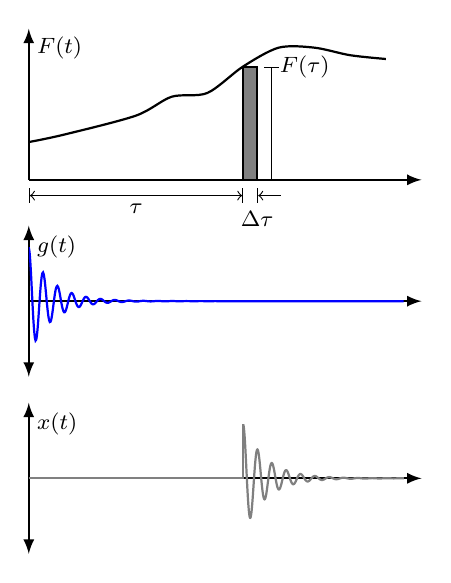
\begin{tikzpicture}[scale=1]
	\footnotesize
\begin{axis}[
	at = {(0,0cm)},
	width=6.57cm,
	height=3.5cm,
	xmax=5.5,
	ymax=4,
	ymin=0,  
	axis lines=left, xtick=\empty, ytick=\empty,axis lines=middle,axis line style = {thick,-latex}]
	
	\node at (axis cs:0,0) [anchor=north east] {$0$};
	\draw [thick,fill = gray] (axis cs: 3,0) rectangle (axis cs: 3.2, 2.99);
	%			\draw [thick,fill = gray!50!white] (axis cs: 3.2,0) rectangle (axis cs: 3.4, 3.2);	
	\draw [|-|] (axis cs: 3.4, 0)  -- (axis cs: 3.4, 3) node [pos=1, right] {$F(\tau)$};
	
	
	\addplot [thick, smooth] coordinates {(0, 1)  (0.5, 1.2)  (1.5, 1.7)  (2, 2.2)  (2.5, 2.3)  (3, 3)  (3.5, 3.5)  (4, 3.5)  (4.5, 3.3) (5, 3.2)};
	\node at (axis cs: 0, 3.5) [right] {$F(t)$};
\end{axis}

\draw [|<->|] (0,-0.2) -- (2.725,-0.2)  node [below, pos=0.5] {$\tau$};
\draw [|<-] (2.9,-0.2) -- (3.2,-0.2)  node [below, pos=0.5] {};
\node at (2.9,-0.5) [] {$\Delta \tau$};

\begin{axis}[
	at = {(0,-2.5cm)},
	width=6.57cm,
	height=3.5cm,
	xmax=5.5,
	ymax=1.4,
	ymin=-1.4,  
	samples=500,
	axis lines=left, xtick=\empty, ytick=\empty,axis lines=middle,axis line style = {thick,-latex},
	y axis line style = {thick,latex-latex}]
	
	\def\wn{5*2*pi};
	\def\xo{1};
	\def\dxo{0};		
	\def\zEta{0.1};
	\def\wdd{sqrt(1-\zEta^2)*\wn};
	\def\Phii{rad(atan(\dxo/(\wdd*\xo)))};
	
	\addplot[blue, thick, domain=0:5.25] (x, {sqrt(\xo^2+(\dxo/\wdd)^2) * cos(deg(\wdd*x- \Phii)) * exp(-\zEta*\wn*x)});
	\node at (axis cs: 0, 1) [right] {$g(t)$};
\end{axis}


\begin{axis}[
	at = {(0,-4.75cm)},
	width=6.57cm,
	height=3.5cm,
	xmax=5.5,
	ymax=1.4,
	ymin=-1.4,  
	samples=500,
	axis lines=left, xtick=\empty, ytick=\empty,axis lines=middle,axis line style = {thick,-latex},
	y axis line style = {thick,latex-latex}]
	
	\def\wn{5*2*pi};
	\def\xo{1};
	\def\dxo{0};		
	\def\zEta{0.1};
	\def\wdd{sqrt(1-\zEta^2)*\wn};
	\def\Phii{rad(atan(\dxo/(\wdd*\xo)))};
	
	\addplot[gray, thick, xshift=77.5,domain=0:2.25] (x, {sqrt(\xo^2+(\dxo/\wdd)^2) * cos(deg(\wdd*(x)- \Phii)) * exp(-\zEta*\wn*x)});
	\addplot [gray, thick] coordinates {(0, 0)  (3., 0)  (3., 1)};
	\node at (axis cs: 0, 1) [right] {$x(t)$};
	\node at (axis cs: 3.4, 3)  {$g(t-\tau)$};
\end{axis}
\end{tikzpicture}

\end{document}